%!TEX root = ../nwoods_thesis.tex

\chapter{Analysis Strategy}

\section{Background Estimation}
Reducible backgrounds for four-lepton events typically have two prompt leptons and two other objects---typically jet fragments, sometimes photons---which are misidentified as prompt leptons.
The largest source of background contamination is from evens in which a {\PZ} boson is produced in association with a photon and a jet, a leptonically-decaying $\PW$ boson and a jet, or two jets.
There is also a contribution from {\TTbar} events in which both top quarks decay to a lepton, a neutrino, and a {\Pqb}~quark jet.
For simplicity, the two sets of processes are not treated separately in what follows, and are collectively labeled ``$\PZ+\PX$'' events.

The contributions of the reducible backgrounds to the selected four-lepton signal samples are evaluated using the tight-to-loose ``fake rates'' method, described more fully in Ref.~\cite{Chatrchyan:2013mxa}.
In this procedure, the likelihood of a nonprompt (``fake'') object to be misidentified as a prompt lepton is estimated and applied to control regions enriched with $\PZ+\PX$ events to estimate their contribution to the signal region.
The lepton misidentification rate $f_\ell\left(\pt^\ell, \eta^\ell\right)$ is measured from a sample of $\PZ + \ell_\text{fake}$ events, where the {\PZ} candidate is selected as in the signal region but with $\left| m_{\ell\ell} - m_\PZ \right| < 10\GeV$, and the $\ell_\text{fake}$ object is a lepton candidate that passes relaxed ID requirements as defined in Section~\ref{sec:looseID}, with no isolation or tight ID requirements applied.
Events with three prompt leptons can contaminate this control region, because the {non-\PZ} lepton is assumed fake.
To avoid the resulting bias in the misidentification rate, the contribution of $\WZ \to 3\ell\nu$ to the $\PZ+\ell_\text{fake}$ sample is estimated from a simulated sample and subtracted.

The misidentification rate is defined as the fraction of $\ell_\text{fake}$ candidates which pass full lepton identification and isolation critera, in bins of $\pt$ and $\eta$.
One should note that this is not a probability in the usual sense, and there is not a simple physical interpretation of these misidentification rates.
Figure~\ref{fig:fakerates} shows the misidentification rates for electrons and muons separately as a function of {\pt} and $\eta$.

\begin{figure}[htbp]
  \begin{center}
    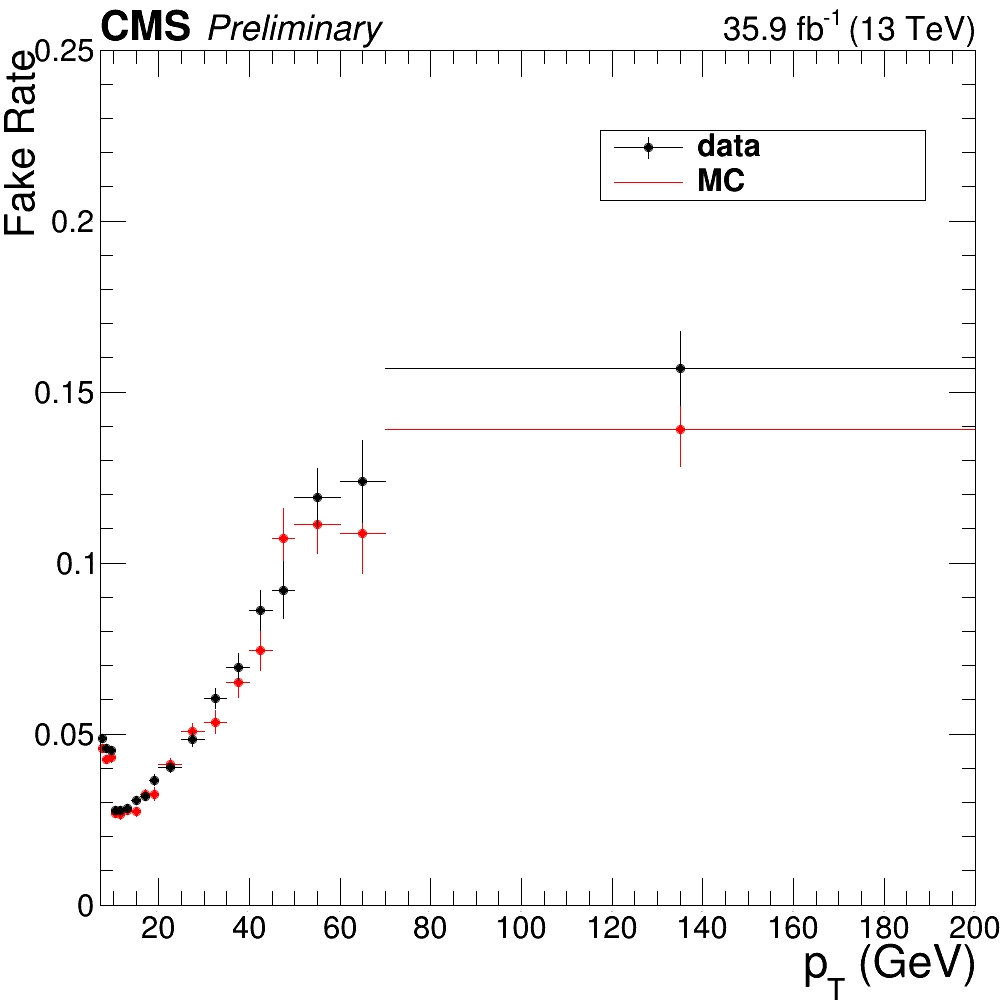
\includegraphics[width=0.35\textwidth]{methods/eFakeRate_pt.png}
    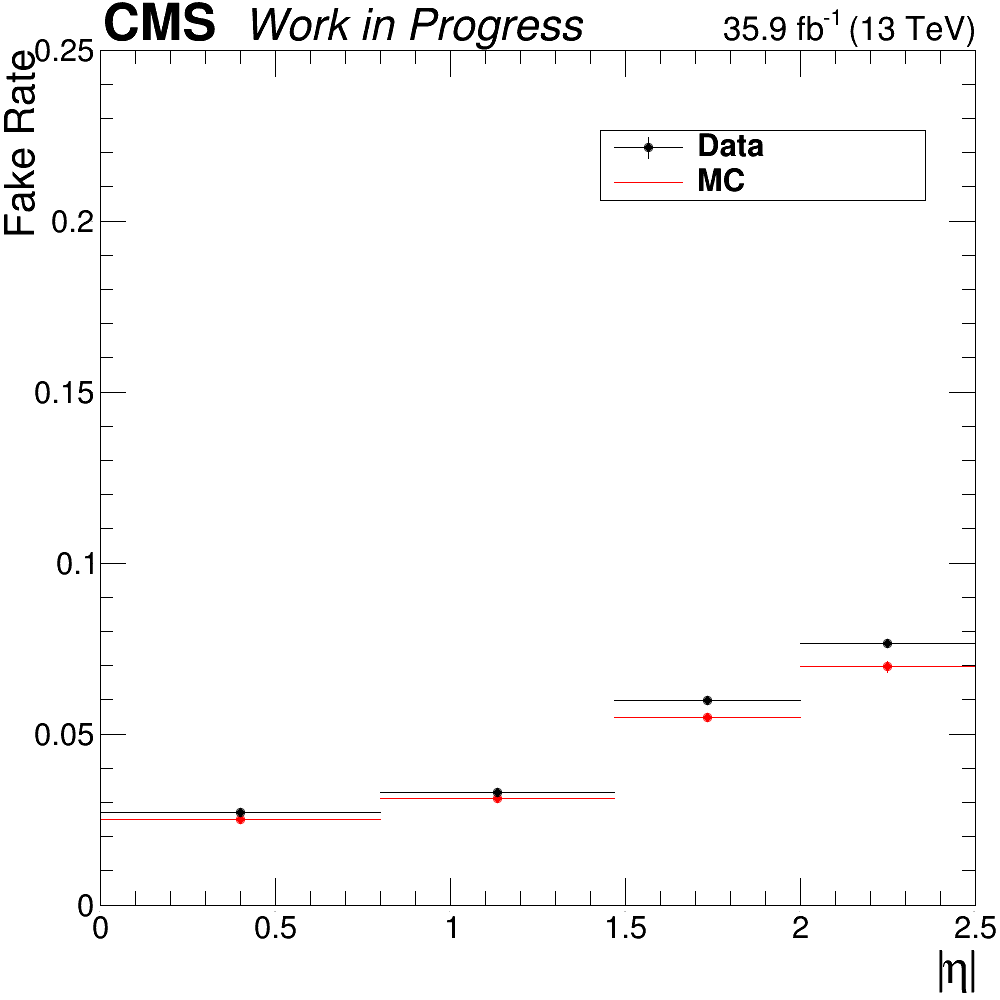
\includegraphics[width=0.35\textwidth]{methods/eFakeRate_eta.png} \\
    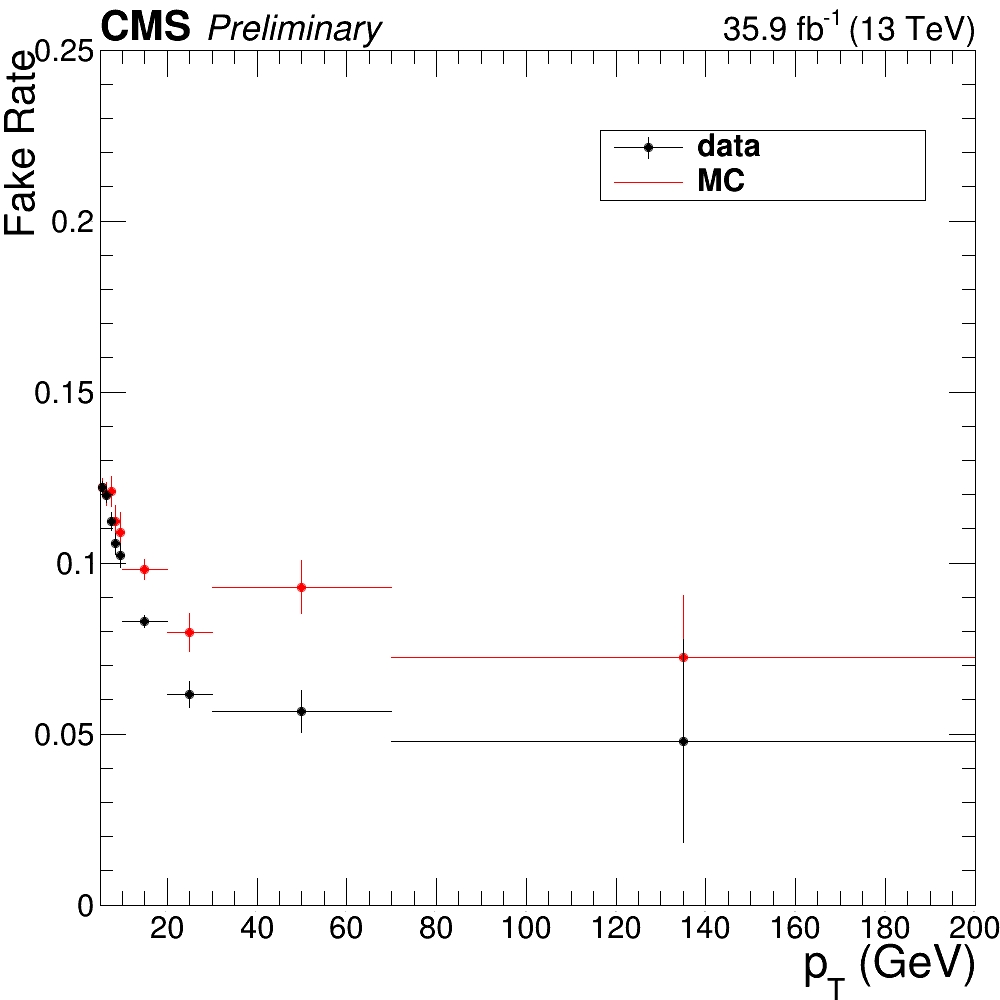
\includegraphics[width=0.35\textwidth]{methods/mFakeRate_pt.png}
    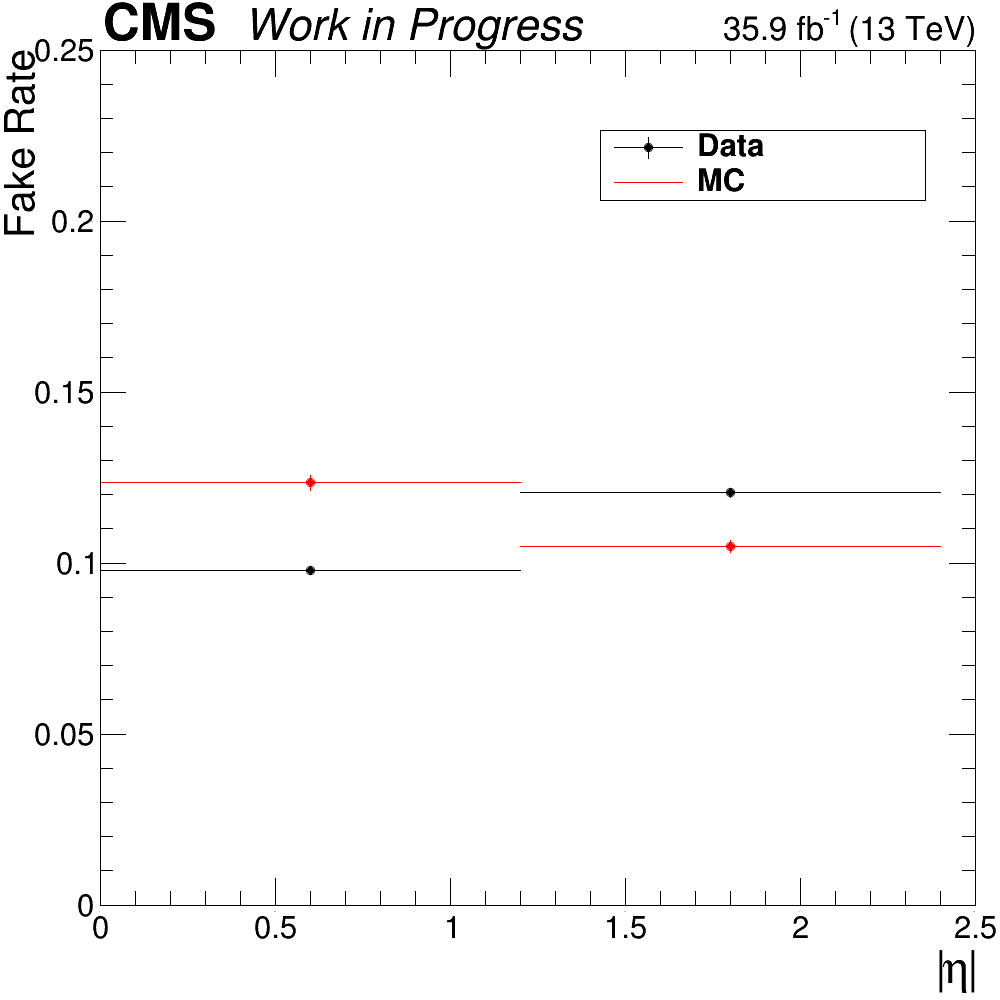
\includegraphics[width=0.35\textwidth]{methods/mFakeRate_eta.png}
    \caption[Misidentification rates for electrons and muons]{
      Fake rate for electrons~(top) and muons~(bottom) as a function of $\pt$~(left) and $\eta$~(right).
      }\label{fig:fakerates}
  \end{center}
\end{figure}

To estimate the total reducible background yield, the misidentification rates are applied to two $\PZ+\PX$ enriched control samples, each containing a {\PZ}~boson candidate passing all signal region requirements plus two more lepton candidates which pass the relaxed identification criteria and would make a second passing {\PZ} boson candidate except that one or both fail the full identification or isolation criteria.
The sample with one failing lepton, called the ``3P1F'' sample for ``3 prompt 1 fake,'' covers the contribution from {\WZ} events, while the sample with both leptons in the second {\PZ} boson failing (``2P2F'') covers $\PZ+\text{jets}$ and {\TTbar} events.
Both have the contribution from {\ZZ} events in which one or two prompt leptons fail identification or isolation criteria removed based on simulated samples.
The fake object transfer factor
\begin{equation}
  F_\ell\left(\pt^\ell,\eta^\ell\right) = \frac{f_\ell\left(\pt^\ell, \eta^\ell\right)}{1 - f_\ell\left(\pt^\ell, \eta^\ell\right)}
\end{equation}
is the ratio of nonprompt objects passing the relaxed and full selection criteria, and thus serves as an extrapolation factor between control sample yields and signal sample yields.

The total reducible background yield is thus
\begin{equation}\label{eq:bkgYield}
  N_\text{bkg} = \sum_{\ell \in \text{3P1F}} F_\ell\left(\pt^\ell,\eta^\ell\right) - \sum_{\ell_1,\ell_2 \in 2P2F} F_{\ell_1}\left(\pt^{\ell_1},\eta^{\ell_1}\right)F_{\ell_2}\left(\pt^{\ell_2},\eta^{\ell_2}\right),
\end{equation}
where subtraction of signal contamination is implicit.
The minus sign in Eq.~\ref{eq:bkgYield} prevents double-counting of $\PZ+2\text{jets}$ events in which one jet fragment is misidentified.

There are also irreducible background contributions from {\TTZ} and {\WWZ} events, which can have four prompt leptons.
Expected yields for these processes are taken from simulation.



\section{Systematic Uncertainties}

Systematic uncertainties for trigger efficiency are taken to be the difference between trigger efficiencies in data and in simulated events, found to be around 2\% of the final event yield.
Because leptons in $\PZ \to 4\ell$ events generally have lower $\pt$, the uncertainty increases to 4\% for $\PZ \to 4\Pe$ events.
In both data and simulated events, trigger efficiencies are found with a tag-and-probe technique~\cite{CMS:2011aa}, performed on four-lepton events.

The lepton identification and isolation efficiencies in simulation are corrected with scaling factors derived with the tag-and-probe method, performed on a sample of $\PZ \to \ell^+\ell^-$ events.
To find the uncertainties associated with these corrections, the total yield is recomputed with the scaling factors varied up and down by the tag-and-probe uncertainties, treating all bins as correlated.
The uncertainties in the $\ZZ \to 4\ell$ yield associated with the tag-and-probe results are found to be 6\% in the $4\Pe$ final state, 3\% in the $2\Pe2\Pm$ final state, and 2\% in the $4\Pm$ final state.
Leptons in $\PZ \to 4\ell$ events tend to have lower {\pt}, and the tag-and-probe samples for low-$\pt$ leptons are smaller and more contaminated with nonprompt objects, so the uncertainties are larger; they are found to be 10\%, 6\%, and 7\% for the $4\Pe$, $2\Pe\Pm$, and $4\Pm$ final states, respectively.

The uncertainty on the LHC integrated luminosity of the data sample is 2.5\%.

The uncertainty on lepton fake rates is taken to be 40\%, which includes both statistical uncertainty and systematic uncertainties associated with the loosened lepton selections used and the differences in the underlying physics processes between events in the $3\ell$ and $4\ell$ control samples.
Statistical uncertainties arising from the limited size of the $\PZ+\PX$ control samples is also included as a systematic uncertainty on the background yield.
The total uncertainty on the background yield varies by channel but is below 1\% of the expected total yield.

Uncertainties due to the effect of QCD scale on the $\ZZ \to 4\ell$ acceptance are evaluated with {\POWHEG} and {\MCFM}, by varying the QCD scales up and down by a factor of two with respect to the default $\mu_R = \mu_F = m_{\ZZ}$.
Parametric  uncertainties (PDF$+ \alpha_s$) are evaluated according to the \textsc{pdf4lhc} prescription in the acceptance calculation~\cite{Butterworth:2015oua}, and with \textsc{nnpdf3.0} in the cross section calculations.
An additional theoretical uncertainty arises from scaling the $\Pq\Paq \to \ZZ$ and $\Pg\Pg \to \ZZ$ simulated samples to their NNLO and NLO predicted cross sections, respectively.
The corresponding change in the acceptance, 1.1\%, is added to the previous theoretical errors in quadrature.

Systematic uncertainties on expected signal yield are summarized in Table~\ref{tab:systematics}.
To obtain uncertainties in computed quantities such as cross sections, the inputs are varied separately for each source and the calculation is fully redone.
For differential cross section and other shape uncertainties, the variations across bins are taken to be fully correlated for each uncertainty source.
Lepton and jet momentum scale and resolution uncertainties are taken to be trivial for the overall yield, but they are considered among the shape uncertainties.

\begin{table}[htbp]
  \centering
  \caption[Systematic uncertainties on the total yield]{
    The contributions of each source of signal systematic uncertainty in the total yields.
    The integrated luminosity uncertainty and the PDF and scale     uncertainties are considered separately.
    All other uncertainties are added in quadrature into a single systematic uncertainty.
    Uncertainties that vary by decay channel are listed as a range.
  }\label{tab:systematics}
  \begin{tabular}{lcc}
    \toprule
    Uncertainty               & $\PZ  \to  4\ell$ & $\ZZ  \to  4\ell$  \\
    \midrule
    Lepton efficiency         & 6--10\%           & 2--6\%             \\
    Trigger efficiency        & 2--4\%            & 2\%                \\
    MC statistics             & 1--2\%            & 0.5\%              \\
    Background                & 0.6--1.3\%        & 0.5--1\%           \\
    Pileup                    & 1--2\%            & 1\%                \\
    \midrule
    PDF                       & 1\%               & 1\%                \\
    QCD Scales                & 1\%               & 1\%                \\
    \midrule
    Integrated luminosity     & 2.5\%             & 2.5\%              \\
    \bottomrule
  \end{tabular}
\end{table}



\section{Fiducial and Total Cross Section Calculation}

Inclusive cross section measurements can be treated as simple binned counting experiments, where the bins are the three decay channels ($4\Pe, 2\Pe2\Pm$, and $4\Pm$).
If $\nu$ events are expected in a given bin, the probability of observing $n$ events is given by the Poisson distribution,
\begin{equation}\label{eq:poisson}
  f\left(n; \nu\right) = e^{-\nu}\frac{\nu^{n}}{n!}.
\end{equation}
In a particle physics analysis like this one, $\nu$ takes the form
\begin{equation}\label{eq:expectedYield}
  \nu = \nu_s\left(\nuisS\right) + \nu_b\left(\nuisB\right) = \mu\left(\nuisS\right) \lumiL_\textit{int} \sigma_\textit{SM} \epsilon + \nu_b\left(\nuisB\right)
\end{equation}
where $\nu_s$ and $\nu_b$ are respectively the expected signal and background yields, $\sigma_\textit{SM}$ is the standard model expectation for the cross section of the signal process and $\epsilon$ is our efficiency for detecting and identifying its events.
The signal and background nuisance parameter vectors $\nuisS$ and $\nuisB$ represent hidden quantities that we do not measure directly but which affect our yields, i.e.\ systematic effects.
The signal strength $\mu$ compares our expectation to what we actually measure:
\begin{equation}\label{eq:signalStrength}
  \mu = \frac{\sigma_\textit{meas}}{\sigma_\textit{SM}}.
\end{equation}

Of the variables in Eqs.~\ref{eq:poisson} and~\ref{eq:expectedYield},  $\sigma_\textit{SM}$ is known from theoretical calculations, and $\epsilon$ is determined from simulation.
The CMS detector is designed to measure $n$, $\nu_b$, and $\lumiL_\textit{int}$, and inferring $\sigma_\textit{meas}$ is a matter of working backwards to the most likely value of the signal strength $\mu$ given the observed data.
Then the measured cross section is simply
\begin{equation}\label{eq:xsecCalculation}
  \sigma_\textit{meas} = \mu\sigma_\textit{SM}.
\end{equation}
One interesting feature of this method is that $\sigma_\textit{SM}$ is used in the calculation of $\mu$ (Eq.~\ref{eq:expectedYield}) and in the final cross section (Eq.~\ref{eq:xsecCalculation}) in such a way that it cancels out, and in fact anything proportional to the true cross section may be used.
In practice, this means that the order at which $\sigma_\textit{SM}$ is calculated does not matter to the extent that higher order corrections to the kinematics of the events do not affect $\epsilon$.


\subsection{Signal Strength Extraction}

The signal strength is found by the method of maximum likelihood~\cite{Olive:2016xmw,bohm2010introduction}.
The likelihood function is the product of the probability distributions across all bins,
\begin{equation}
  L\left(\nuisS,\nuisB\right) = \prod_\textit{bins} f\left(n; \nu\left(\nuisS,\nuisB\right) \right).
\end{equation}
The most likely value of $\nu$ is the one that maximizes $L$.
In practice, $\log L$ is typically maximized instead because it is easier to work with,
\begin{equation}
  \frac{\partial^2 \log L}{\partial \nuisS \partial \nuisB} = 0.
\end{equation}
This maximization is performed simultaneously for all bins, yielding a single signal strength across all channels.
Systematic uncertainties enter as log-normal constraints imposed on the fit, encoded in $\nuisS$ and $\nuisB$.
The fit is performed numerically.


\subsection{Total ZZ Cross Section and \texorpdfstring{$\mathrm{Z} \to 4\ell$}{Z to 4l} Branching Fraction}

Once the fiducial cross section has been found, it can be used to find the total cross section, subject only to the constraint that both {\PZ} bosons be in the {60--120\GeV} mass range.
The fiducial cross section is related to the total cross section by an acceptance factor $\mathcal{A}$ which accounts for $\ZZ \to 4\ell$ events outside the fiducial definition, and two factors of the {\PZ} branching fraction $\mathcal{B}\left(\PZ \to 2\ell\right)$ to account for all other final states:
\begin{equation}
  \sigma_\mathit{fid} = \mathcal{A} \sigma_\mathit{tot} \left( \mathcal{B}\left(\PZ \to 2\ell\right) \right)^2.
\end{equation}
The acceptance factor is independent of any experimental effects and can be calculated from Monte Carlo events at generator level.
The {\PZ} branching fraction is well known~\cite{Olive:2016xmw}.

The total {\PZ} cross section is better measured in the $2\ell$ channel, because the larger branching fraction yields samples several orders of magnitude larger than the $\PZ \to 4\ell$ sample used here.
It is therefore more interesting to use $\sigma_\textit{fid}\left(\PZ \to 4\ell\right)$ for a measurement of the four-lepton branching fraction $\mathcal{B}\left(\PZ \to 4\ell\right)$.
After applying the acceptance correction to obtain $\sigma_\textit{tot} \left(\PZ \to 4\ell\right) = \sigma_\textit{fid}\left(\PZ \to 4\ell\right) / \mathcal{A}$, the four-lepton branching fraction is given by
\begin{equation}
  \mathcal{B}\left(\PZ \to 4\ell\right) = \frac{\sigma_\textit{tot} \left(\PZ \to 4\ell\right)} {\mathcal{C}^{\text{60--120}}_{\text{80--100}} \, \sigma \left(\PZ \to 2\ell\right)}\mathcal{B}\left(\PZ \to 2\ell\right),
\end{equation}
where $\sigma \left(\PZ \to 2\ell\right)$ is the dileptonic {\PZ} cross section in the {60--120\GeV} mass range and $\mathcal{C}^{\text{60--120}}_{\text{80--100}}$ corrects for the fact that $\sigma\left(\PZ \to 4\ell\right)$ is found in a mass range of {80--100\GeV}.



\section{Differential Cross Sections}

Measurement of a differential fiducial cross section is also a problem of finding the most likely true distribution given observed yields in multiple bins, estimated background yields, and detector effects understood through simulation.
Unlike the inclusive cross section, however, finite detector resolution leads to ``smearing'' effects that cause events to migrate across bins, in addition to the same inefficiencies.
The mean detector-level distribution $\vec{\delta}$ is related to the true distribution $\vec{\theta}$ by a response matrix $\mathbf{R}$:
\begin{equation}
  \vec{\delta} = \mathbf{R}\vec{\theta}.
\end{equation}
The observed distribution in data $\vec{d}$ is sampled from the Poisson distribution with mean $\vec{\delta}$ independently in each bin.
CMS simulation software is sufficiently sophisticated to give a good estimate of $R$.
Note that the case of bins with no migration, as in the inclusive cross section measurement, is the special case where $\mathbf{R}$ is diagonal.

If $\mathbf{R}$ is square and invertible, the maximum likelihood estimate (MLE) of the true distribution, $\hat{\vec{\theta}}$, is given by
\begin{equation}\label{eq:unfoldingMLE}
  \hat{\vec{\theta}} = \mathbf{R}^{-1}\vec{d}.
\end{equation}
Even when $\mathbf{R}$ is invertible, however, it is frequently ill-conditioned, giving $\hat\vec\theta$ unphysical features like large bin-by-bin fluctuations or even negative bins as a consequence of the stochastic nature of $\vec{d}$.
It is therefore necessary to use a more sophisticated procedure to ensure the differential cross section distributions obey physics-inspired constraints.

\subsection{Unfolding}

The technique used here is an iterative frequentist method developed in high energy physics by D'Agostini~\cite{DAgostini:1994fjx} and independently in other fields~\cite{Dempster:10.2307/2984875,Lucy:1974AJ,Richardson:72,Shepp:4307558}.
At iteration $k$, bin $j$ of the predicted true distribution is set based on its expected contribution to all other bins, weighted by the observed data yield in each:
\begin{equation}
  \begin{split}
    \theta_j^{(k+1)} & = \sum_i \mathbf{R}_{ij} \theta_j^{(k)} \frac{d_i}{\delta_i} \\
    & = \sum_i \mathbf{R}_{ij} \theta_j^{(k)} \frac{d_i}{\sum_m \mathbf{R}_{im} \theta_m^{(k)}}.
  \end{split}
\end{equation}
After several iterations, $\vec{\theta}^{(k)}$ depends only weakly on the ansatz $\vec{\theta}^{(0)}$.

The sequence will converge to the MLE for any non-pathological choice of $\vec{\theta}^{(0)}$~\cite{vardi1985}, but again the MLE often displays unphysical behavior.
If $\vec{\theta}^{(0)}$ is strictly positive, $\vec{\theta}^{(k)}$ will be strictly positive for all $k$, and in this case $\hat{\vec{\theta}}$ (as defined in Eq.~\ref{eq:unfoldingMLE}) will be the asymptotic unfolded distribution as long as it is also strictly positive.
Choosing a smooth function for $\vec{\theta}^{(0)}$ will generally lead to smooth $\vec{\theta}^{(k)}$ for small $k$; typical choises include a flat initial distribution and the truth-level distribution used to construct $\mathbf{R}$ (used in this analysis).
What constitutes ``small'' $k$ depends on the condition of $\mathbf{R}$, but for most physics distributions of interest, including all those used in this analysis, nonphysical fluctuations do not arise until after $\vec{\theta}^{(k)}$ is close to convergence.
Full regularization is therefore imposed by ceasing iteration early.
For all distributions shown here, stopping after four iterations was found to give acceptable bias-variance tradeoff.

\subsection{Uncertainties}

The largest uncertainties in the unfolded distributions arise from the unfolding procedure itself, which can inflate statistical uncertainties present in the detector-level distributions.
The correlation matrix which gives the full uncertainty---considered the statistical uncertainty of the unfolded distribution---does not have a closed form due to the nonlinearity of the method.
The covariance matrix is therefore estimated by propagating the statistical error of the inputs at each iteration of the method, as laid out in Ref.~\cite{DAgostini:1994fjx} and improved in Ref.~\cite{Adye:2011gm}.
This procedure does not account for the bias introduced by regularization, but this is expected to be negligible relative to other systematic uncertainties for the well-modeled processes studied here.

Most systematic uncertainties are propagated through unfolding by recomputing the response matrix with the training sample shifted or reweighted to reflect a $1\sigma$ shift in the quantity in question.
The uncertainty related to that quantity is taken to be the resulting shape difference in the final unfolded distribution.
Systematic uncertainties are negligible compared to statistical uncertainties in most bins.


\section{VBS Signal Extraction}
BDTs and other hip things



\section{Anomalous Gauge Coupling Searches}
